% This file creates an a0 portrait poster (3 feet wide X 4 feet high)
% Written by Jennifer de Kleine for her poster for the MITACS AGM 2003.
% Based on template file written by Graeme, 2001-03 based on his SOC poster.
% See discussion and documentation at
% <http://www.astro.gla.ac.uk/users/norman/docs/posters/> 
%
% $Id: poster-template-portrait.tex,v 1.2 2002/12/03 11:25:55 norman Exp $


% We switch to portrait mode. This works as advertised.

\documentclass[a0,landscape]{a0poster}  % 4 feet wide X 3 feet high

% You might find the 'draft' option to a0 poster useful if you have
% lots of graphics, because they can take some time to process and
% display. (\documentclass[draft]{a0poster})

% Switch off page numbers on a poster, obviously, and section numbers too.
\pagestyle{empty}
\setcounter{secnumdepth}{0}

% The textpos package is necessary to position textblocks at arbitary 
% places on the page.
\usepackage[absolute]{textpos}
%\usepackage{subfigure}

% Graphics to include graphics. Times is nice on posters, but you
% might want to switch it off and go for CMR fonts.
\usepackage[final]{graphics}
\usepackage{graphicx,wrapfig,amsfonts, eso-pic,url}
\usepackage{amsmath,amsfonts,amssymb,amsthm,mathtools,enumitem,blkarray}
\usepackage[justification=centering]{caption}
\usepackage{algorithmicx,algpseudocode}
\usepackage{stmaryrd}
\algrenewcommand\algorithmicforall{\textbf{for each}}
\algrenewcommand{\algorithmiccomment}[1]{// #1}

%BEGIN GARY TIKZ PRE

%\usepackage[svgnames]{xcolor}
\usepackage{tikz}
%\usetikzlibrary{decorations.markings}
%\pagestyle{empty}

\pgfdeclarelayer{edgelayer}
\pgfdeclarelayer{nodelayer}
\pgfsetlayers{edgelayer,nodelayer,main}

\tikzstyle{none}=[inner sep=0pt]
\definecolor{hexcolor0xf81e1c}{rgb}{0.973,0.118,0.110}
\definecolor{hexcolor0x3c00ff}{rgb}{0.235,0.000,1.000}

\tikzstyle{vertex}=[circle, fill=white,draw=black, scale=0.55]
\tikzstyle{whitevertex}=[circle,fill=white,draw=black, scale = 0.5]
\tikzstyle{redvertex}=[circle,fill=hexcolor0xf81e1c,draw=black, scale = 0.5]
\tikzstyle{bluevertex}=[circle,fill=hexcolor0x3c00ff,draw=black, scale = 0.5]
\tikzstyle{greenvertex}=[circle,fill=green,draw=black, scale=0.5]
\tikzstyle{purplevertex}=[circle,fill=magenta,draw=black, scale=0.5]
\tikzstyle{yellowvertex}=[circle,fill=yellow,draw=black, scale=0.5]
\tikzstyle{grayvertex}=[circle,fill=gray,draw=black, scale=0.5]
\tikzstyle{blackvertex}=[circle,fill=black,draw=black, scale=0.5]
\tikzstyle{cyanvertex}=[circle,fill=cyan,draw=black, scale=0.5]

\tikzstyle{textbox}=[rectangle,fill=none,draw=none]
\tikzstyle{box}=[rectangle,fill=none,draw=black]

\tikzstyle{arc}=[black, ->]
\tikzstyle{grayarc}=[gray, ->]
\tikzstyle{bluearc}=[blue, ->]
\tikzstyle{grayedge}=[draw=gray]
\tikzstyle{blueedge}=[draw=blue, thick]
\tikzstyle{rededge}=[draw=red, thick]
\tikzstyle{purpleedge}=[draw=magenta, very thick]
\tikzstyle{greenedge}=[draw=green, thick]
\tikzstyle{blackedge}=[draw=black, thick]
\tikzstyle{dashededge}=[draw=black, dashed]
\tikzstyle{edge}=[draw=black]

\tikzstyle{10circle}=[circle, scale=10.0,draw=black]
\tikzstyle{10oval}=[ellipse, scale=10.0,draw=black]

%END GARY'S TIKZ PRE


\newcommand{\F}{\mathbb{F}}
\newcommand{\Fm}{\mathbb{F}_{2^m}}
\newcommand{\E}{\mathcal E}
\newcommand{\Z}{\mathbb{Z}}
\newcommand{\Q}{\mathbb{Q}}
\newcommand{\M}{\mathcal M}
\newcommand{\Cone}{\mathcal C}
\newcommand{\N}{\mathbb{N}}
\newcommand{\bm}[1]{\mathbf{#1}}

\def\tr{{\rm Tr}}
\def\Tr{{\rm Tr}}

\newcommand{\R}{\mathbb{R}}
\newcommand{\C}{\mathbb{C}}
\newcommand{\Zd}{\mathbb{Z}_d}
\newcommand{\om}{\omega}
\newcommand{\lam}{\lambda}
\newcommand{\QED}{\hfill $\Box$ \hfill \\}

\newcommand{\divides}{\ \big|\ }

\theoremstyle{plain}
\newtheorem{lem}{Lemma}
\newtheorem{thm}{Theorem}
\newtheorem{theorem}{Theorem}
\newtheorem{cor}{Corollary}
\newtheorem{prop}{Proposition}
\newtheorem{defn}{Definition}
\newtheorem{conj}{Conjecture}
\renewcommand\refname{}
% These colours are tried and tested for titles and headers. 
\usepackage{color}
\definecolor{DarkRed}{rgb}{0.5,0.0,0.0} 
\definecolor{Black}{rgb}{0,0,0} 
\definecolor{DarkBlue}{rgb}{0.1,0.1,0.5} % very dark, almost looks like black
\definecolor{Red}{rgb}{0.9,0.0,0.1}
\definecolor{Blue}{rgb}{0.1,0,0.8} % I designed this for Maple output
\definecolor{Auburn}{rgb}{0.443, 0.184, 0.149}
\definecolor{Saphire}{rgb}{0.0314, 0.145, 0.404}
\definecolor{Burgundy}{rgb}{0.6,0,0.125}
\definecolor{DarkOrchid}{rgb}{0.75,0,0.25}

\definecolor{LightBlue}{rgb}{0.0,0.5,1.0} % I designed this for Background
\definecolor{LightPink}{rgb}{1,0.8,0.8} %background?

\definecolor{Grey}{rgb}{0.5,0.5,0.5} % a very light grey
\definecolor{Green}{rgb}{0,0.5,0.1} % 


% background color
%\pagecolor{LightBlue}

% see documentation for a0poster class for the size options here
% you can define your own headers, vary the colour and size as you like
\let\Textsize\normalsize
\def\Hugehead#1{\noindent{\Huge\color{Saphire} #1}}
\def\LARGEhead#1{\noindent{\LARGE\color{DarkBlue} #1}}
\def\Largehead#1{\noindent{\Large\color{DarkBlue} #1}}
\def\largehead#1{\noindent{\large #1}}
\def\Title#1{\noindent{\VeryHuge\color{DarkBlue} #1}}
   \def\MapleInput#1#2#3{\begin{textblock}{7}(#1,#2) \noindent{\color{Red} $>$ {\bf\tt #3}}\end{textblock}}
\def\MapleOutput#1#2#3{\begin{textblock}{7}(#1,#2){\color{Blue} #3}\end{textblock}}
%\def\MapleOutputC#1{\begin{center}{\color{Blue} #1}\end{center}}

% Set up the grid
%
% Note that [40mm,40mm] is the margin round the edge of the page --
% it is _not_ the grid size. That is always defined as 
% PAGE_WIDTH/HGRID and PAGE_HEIGHT/VGRID. In this case we use
% 15 x 25. This gives us a wide central column for text (7 grid
% spacings) and two narrow columns (3 each) at each side for 
% pictures, separated by 1 grid spacing.
%
% Note however that texblocks can be positioned fractionally as well,
% so really any convenient grid size can be used.

\TPGrid[40mm,40mm]{26}{15}  % 3 - 1 - 7 - 1 - 3 Columns
                            % I am only using two columns: 4.5 - 1 - 9.4
                            % you can do whatever you like

% Mess with these as you like
\parindent=0pt
%\parindent=1cm
\parskip=0.5\baselineskip

\begin{document}

% Understanding textblocks is the key to being able to do a poster in
% LaTeX. In
%
%    \begin{textblock}{wid}(x,y)
%    ...
%    \end{textblock}
%
% the first argument gives the block width in units of the grid
% cells specified above in \TPGrid; the second gives the (x,y)
% position on the grid, with the y axis pointing down.

% You will have to do a lot of previewing to get everything in the 
% right place.

% TOP PART
\begin{textblock}{20}(10,-0.1)
\baselineskip=3\baselineskip\Title{\color{black}\bf Measuring Chaos}
\end{textblock}

\begin{textblock}{6}(20,-0.5)

  
\includegraphics[]{mathstatslogohorr}

\Large{\textbf{This research was supported by the Jamie Cassels Undergraduate Research Award}}
\end{textblock}

\begin{textblock}{25.5}(0,0.75)
\begin{center}{\Hugehead{\color{black}\bf Andrew Wilson, Supervised by Dr. Anthony Quas}}
\end{center}
\end{textblock}

%\begin{textblock}{5}(11,1.6)
 % \LARGEhead{{\tt \{anjam\}@uvic.ca}}
%\end{textblock}

% I used xfig to create greyline.eps
\begin{textblock}{26}(0,2.2)
 % \resizebox{26\TPHorizModule}{!}{\includegraphics{greyline.eps}}  
\end{textblock}


\begin{textblock}{7}(0,.3)
 % \resizebox{7\TPHorizModule}{!}{\includegraphics{banner1}} 
  
%\begin{textblock}{7}(0,0)
  %\resizebox{7\TPHorizModule}{!}{\includegraphics{banner2}} 
\end{textblock}

%\begin{textblock}{2}(0,0)
 % \resizebox{1.7\TPHorizModule}{!}{\includegraphics{bigsfulogo.eps}} 
%\end{textblock}

\begin{textblock}{2}(3,1.5)

\end{textblock}

\begin{textblock}{1.8}(21,0.1)
%  \resizebox{3\TPHorizModule}{!}{\includegraphics{CMS.eps}}
\end{textblock}

%%%%% START OF CONTENT %%%%%%%
\begin{textblock}{7}(1,1.8)
\Hugehead{What is Chaos?} %\large
\nocite{*}
\end{textblock}

\begin{textblock}{5.5}(0,2.25)
\Large{Roughly speaking, we say that a system is chaotic if it is sensitive to initial
conditions. That is, in a deterministic
system, if small changes are made to an input, we expect to see vastly different outputs.

A `system' can roughly be thought of as a set of points and a map that moves those points around. 

For example: air molecules in the atmosphere and the wind, or the position of the
end of a double pendulum under the influence of gravity. }
\end{textblock}

\begin{textblock}{2}(5.9,2.8)
\begin{figure}
\vspace{-3 mm}
\hspace{8mm}

% Picture of double pendulum, three stages

\vspace{0 mm}
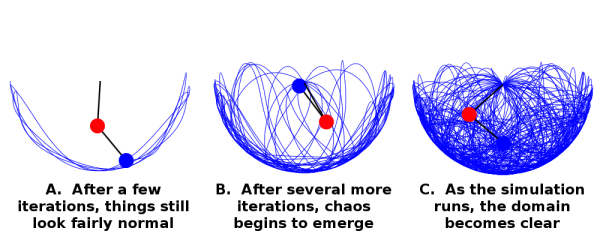
\includegraphics[scale=1]{./Pictures/doublePendulum.png}
\caption{}
\end{figure}
\end{textblock}

\begin{textblock}{7.5}(0,7)

\Hugehead{Modelling Chaos: Dynamical Systems} 
\smallskip

{\Large In order to study chaos, we need models of the systems we would like to investigate. 
How can we abstract some of the previous examples in a way that can be studied mathematically?}

{\Large {\bf Definition:} A Dynamical System is a pair $(X,T)$ where $X$ is a set of points, and $T$ is 
function from $X$ to $X$.}

{\Large Formalizing our first example from before, define $$X=\{\text{air particles in the
atmosphere}\}$$ and $T$ to map an air particle to its position after being acted on by the wind for 
one second.} 

{\Large 

\end{textblock}

\begin{textblock}{5}(0,13.4)
\large {
\begin{center}
\begin{figure}
%\includegraphics[width=150mm,scale=1]{eq.png}
\vspace{-5mm}
\caption{
Caption
}
\end{figure}
\end{center}
}
\end{textblock}


\begin{textblock}{3.5}(4.5,13.7)
\large{Caption}
\end{textblock}

% end column 1

%%%%%%%%%%%%%%%%%%%%%%%%%%%%%%%%%%%%%%%%%%%%%%%%%%%%%%%%%%%%%%%%
%% SECOND COLUMN of MY POSTER---STARTS here
%%%%%%%%%%%%%%%%%%%%%%%%%%%%%%%%%%%%%%%%%%%%%%%%%%%%%%%%%%%%%%%%

\begin{textblock}{8}(8.4,1.8)
\Hugehead{Stable and Unstable Manifolds}
\end{textblock}

\begin{textblock}{8}(8.4,2.25)
\large{

\vspace{-3cm}
\begin{align*}
(1)\text{ } &\text{If } x + y \in K \text{ and } x,y\in C \text{ then } x,y \in K \\
(2)\text{ } &\mathrm{span}\{K\} \text{ has codimension } 1
\end{align*}
A {\bf facet normal} is a vector orthogonal to a facet. 
\end{defn}
%The amounts to a facet normal of a cone $C$ in $\R^k$ is a vector $x$ that is perpendicular to a subspace generated by vectors in the generating set of $C$ of dimension $k-1$
}
\end{textblock}

\begin{textblock}{4}(7.8,4)
\large {
\begin{figure}
\vspace{2mm}
\hspace{30mm}
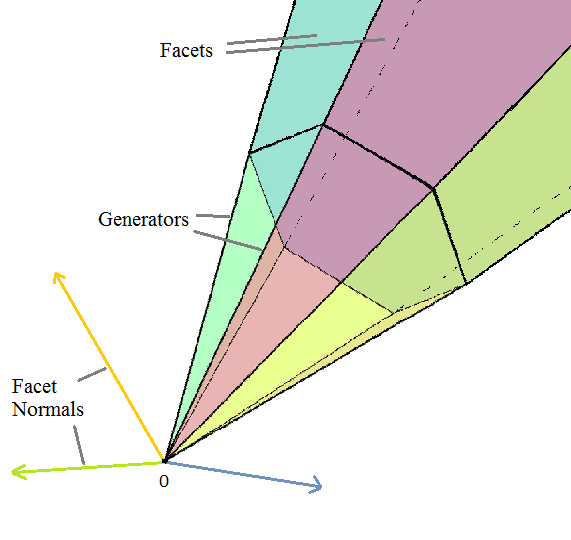
\includegraphics[width=100mm,scale=1]{polyhedralconescew.png}
%\begin{tikzpicture}[scale=1.6, transform shape] 
%\node at ( 3.02 , 0.35){\small{$x_1$}};
%\node at (0.55, 3.75){\small{$x_2$}};\
%\draw [-latex, thick] (0,0) -- (2,1);
%\draw [-latex, thick] (0,0) -- (1,3);
%\draw [-latex, thick] (-2,0) -- (3.5,0);
%\draw [-latex, thick] (0,-1.5) -- (0,4);
%\draw [-latex, red, thick] (0,0) -- (-1,2);
%\draw [-latex, red, thick] (0,0) -- (3,-1);
%\fill[gray!80,nearly transparent] (0,0) -- (1.333,4) -- (3,1.5) -- cycle;
%\node at ( 1.25 , 1.5){$\mathcal{C}_A$};
%\coordinate (O) at (0,0);
%\coordinate (A) at (2,1);
%\coordinate (B) at (1,-2);
%\tkzMarkRightAngle[fill=orange,size=0.8cm,opacity=.4](B,O,A);
%\end{tikzpicture}

\vspace{-5mm}
\caption{
Polyhedral cone \\ in $\R^3$
}

\end{figure}
}
\end{textblock}

\begin{textblock}{5.3}(11.2,3.9)
\large {
Figure 3 depicts the components of a cone in $\R^3$. To investigate the structure of cones this project looked at adjacency between facets. Two facets are {\bf adjacent} if their intersection is a cone in a codimension  $2$ subspace. This is equivalent to two facets being adjacent if for their facet normals $f_1$ and $f_2$, the  orthogonal complement of their sum ($f_1+f_2$) intersected with the original cone has codimension $2$. This is a result of a dimension theorem implying that

\vspace{-1.5cm} $$\text{span}\{F_1\cap F_2\} = \text{span}\{F_1\} \cap \text{span}\{F_2\}.$$ 
}
\end{textblock}

\begin{textblock}{8}(8.4,6.9)
\large{It is clear that in our cone generated by triangles, there are finitely many facets all of which are determined uniquely by their facet normals. Using programming tools we have made a relatively efficient algorithm for classifying the facets by their normals. We have done the calculations for $n=5,6,7, \text{ and }8$, in which there are $10$, $70$, $897$ and, $52367$ facets  respectively. However, the number of facets on these cones grow extremely fast and quickly become impractical; when $n=9$ we have a list of facets that seems to be complete but remains to be proven. }
\end{textblock}

\begin{textblock}{6}(8.4,8.78)
\large{It is important to note that there are isomorphism classes between facets, stemming from redundancy of vertex labeling. For $n=5,6,7,$ and $8$ there are $1$, $4$, $7$, and $19$ respectively and we predict that there are $143$ when $n=9$. Figure 4 shows two facets that represent isomorphism classes. For some more data on these results visit the following links:} \\ (1)  http://oeis.org/A246427 \\(2) http://www.math.uvic.ca/~dukes/facets-tri9.txt 
\end{textblock}

\begin{textblock}{2}(14.6,8.5)
\begin{figure}
\begin{center}


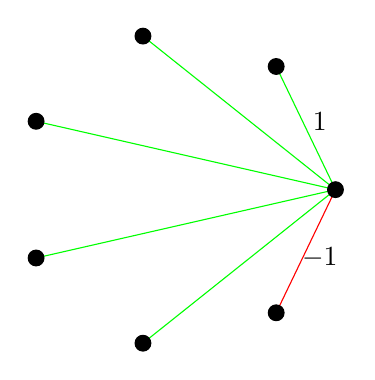
\begin{tikzpicture}[scale=1]
\node at ( 1.802 , 0.868 ){$ 1 $};
\draw[green! 100.0 !red] ( 2.0 , 0.0 )--( 1.247 , 1.564 );
\draw[green! 100.0 !red] ( 2.0 , 0.0 )--( -0.445 , 1.95 );
\draw[green! 100.0 !red] ( 2.0 , 0.0 )--( -1.802 , 0.868 );
\draw[green! 100.0 !red] ( 2.0 , 0.0 )--( -1.802 , -0.868 );
\draw[green! 100.0 !red] ( 2.0 , 0.0 )--( -0.445 , -1.95 );
\node at ( 1.802 , -0.868 ){$ -1 $};
\draw[red! 100.0 !green] ( 2.0 , 0.0 )--( 1.247 , -1.564 );
\filldraw ( 2.0 , 0.0 ) circle [radius=.1];
\filldraw ( 1.247 , 1.564 ) circle [radius=.1];
\filldraw ( -0.445 , 1.95 ) circle [radius=.1];
\filldraw ( -1.802 , 0.868 ) circle [radius=.1];
\filldraw ( -1.802 , -0.868 ) circle [radius=.1];
\filldraw ( -0.445 , -1.95 ) circle [radius=.1];
\filldraw ( 1.247 , -1.564 ) circle [radius=.1];
\end{tikzpicture}
\\
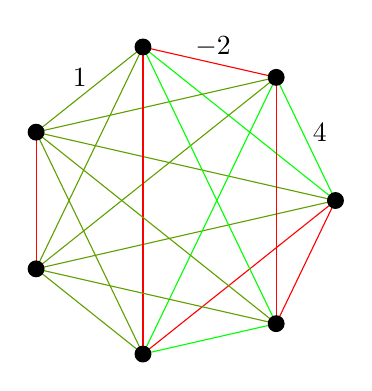
\begin{tikzpicture}[scale=1]
\node at ( 1.802 , 0.868 ){$ 4 $};
\draw[green! 100.0 !red] ( 2.0 , 0.0 )--( 1.247 , 1.564 );
\draw[green! 100.0 !red] ( 2.0 , 0.0 )--( -0.445 , 1.95 );
\node at ( 0.445 , 1.95 ){$ -2 $};
\draw[red! 100.0 !green] ( 1.247 , 1.564 )--( -0.445 , 1.95 );
\draw[green! 62.5 !red] ( 2.0 , 0.0 )--( -1.802 , 0.868 );
\draw[green! 62.5 !red] ( 1.247 , 1.564 )--( -1.802 , 0.868 );
\node at ( -1.247 , 1.564 ){$ 1 $};
\draw[green! 62.5 !red] ( -0.445 , 1.95 )--( -1.802 , 0.868 );
\draw[green! 62.5 !red] ( 2.0 , 0.0 )--( -1.802 , -0.868 );
\draw[green! 62.5 !red] ( 1.247 , 1.564 )--( -1.802 , -0.868 );
\draw[green! 62.5 !red] ( -0.445 , 1.95 )--( -1.802 , -0.868 );
\draw[red! 100.0 !green] ( -1.802 , 0.868 )--( -1.802 , -0.868 );
\draw[red! 100.0 !green] ( 2.0 , 0.0 )--( -0.445 , -1.95 );
\draw[green! 100.0 !red] ( 1.247 , 1.564 )--( -0.445 , -1.95 );
\draw[red! 100.0 !green] ( -0.445 , 1.95 )--( -0.445 , -1.95 );
\draw[green! 62.5 !red] ( -1.802 , 0.868 )--( -0.445 , -1.95 );
\draw[green! 62.5 !red] ( -1.802 , -0.868 )--( -0.445 , -1.95 );
\draw[red! 100.0 !green] ( 2.0 , 0.0 )--( 1.247 , -1.564 );
\draw[red! 100.0 !green] ( 1.247 , 1.564 )--( 1.247 , -1.564 );
\draw[green! 100.0 !red] ( -0.445 , 1.95 )--( 1.247 , -1.564 );
\draw[green! 62.5 !red] ( -1.802 , 0.868 )--( 1.247 , -1.564 );
\draw[green! 62.5 !red] ( -1.802 , -0.868 )--( 1.247 , -1.564 );
\draw[green! 100.0 !red] ( -0.445 , -1.95 )--( 1.247 , -1.564 );
\filldraw ( 2.0 , 0.0 ) circle [radius=.1];
\filldraw ( 1.247 , 1.564 ) circle [radius=.1];
\filldraw ( -0.445 , 1.95 ) circle [radius=.1];
\filldraw ( -1.802 , 0.868 ) circle [radius=.1];
\filldraw ( -1.802 , -0.868 ) circle [radius=.1];
\filldraw ( -0.445 , -1.95 ) circle [radius=.1];
\filldraw ( 1.247 , -1.564 ) circle [radius=.1];
\end{tikzpicture}
\caption{$n=7$ facet examples}
\end{center}
\end{figure}
\end{textblock}

\begin{textblock}{8}(8.4,10.7)
\bigskip
\LARGEhead{Trivial adjacencies of facets}

\large{
For any $n>5$ every unit vector $u = (0,...,0,1,0,...,0)$ orthogonal complement that satisfies the requirements of a facet. We call these facets the {\bf trivial facets}. Computational evidence suggests that for $n>5$ every facet is adjacent to a trivial facet. The main goal of this research was to take steps in proving that all facets are adjacent to a trivial facet for $n>5$.
}

\large{
Every facet $F$ induces a graph of {\bf trivial adjacencies}, a graph that is the sum all the normals to trivial facets adjacent to $F$. Figure 5 shows the adjacency graphs of the facets shown in figure 4. 
}
\end{textblock}


\begin{textblock}{8}(8.4,13.5)
\begin{figure}

\begin{center}
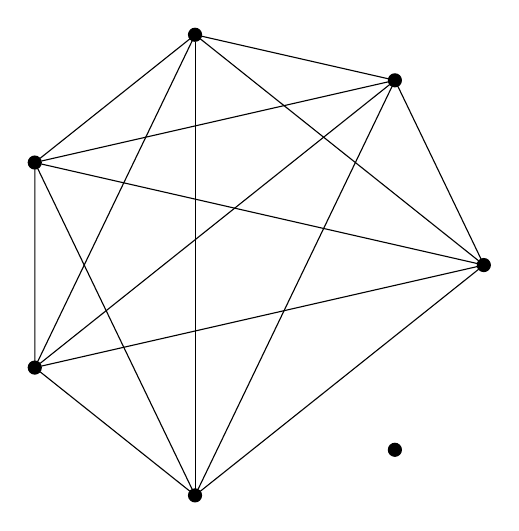
\begin{tikzpicture}[scale = 1.5]
	\begin{pgfonlayer}{nodelayer}
	
	%K_7
		\node [style=blackvertex] (3) at (8.000,0.500) {};
		\node [style=blackvertex] (4) at (7.247,2.064) {};
		\node [style=blackvertex] (5) at (5.555,2.450) {};
		\node [style=blackvertex] (6) at (4.198,1.368) {};
		\node [style=blackvertex] (7) at (4.198,-0.368) {};
		\node [style=blackvertex] (8) at (5.555,-1.450) {};
		\node [style=blackvertex] (9) at (7.247,-1.064) {};

	\end{pgfonlayer}
	\begin{pgfonlayer}{edgelayer}
		
		%K_7
		\draw (3) to (4);
		\draw (3) to (5);
		\draw (3) to (6);
		\draw (3) to (7);
		\draw (3) to (8);
		\draw (4) to (5);
		\draw (4) to (6);
		\draw (4) to (7);
		\draw (4) to (8);
		\draw (5) to (6);
		\draw (5) to (7);
		\draw (5) to (8);
		\draw (6) to (7);
		\draw (6) to (8);
		\draw (7) to (8);
		
	\end{pgfonlayer}
\end{tikzpicture}
\hspace{3cm}
\begin{tikzpicture}[scale = 1.5]
	\begin{pgfonlayer}{nodelayer}
	
	%K_7
		\node [style=blackvertex] (3) at (8.000,0.500) {};
		\node [style=blackvertex] (4) at (7.247,2.064) {};
		\node [style=blackvertex] (5) at (5.555,2.450) {};
		\node [style=blackvertex] (6) at (4.198,1.368) {};
		\node [style=blackvertex] (7) at (4.198,-0.368) {};
		\node [style=blackvertex] (8) at (5.555,-1.450) {};
		\node [style=blackvertex] (9) at (7.247,-1.064) {};

	\end{pgfonlayer}
	\begin{pgfonlayer}{edgelayer}
		
		%K_7
		\draw (3) to (4);
		\draw (3) to (5);
		\draw (4) to (8);
		\draw (8) to (9);
		\draw (9) to (5);
		
	\end{pgfonlayer}
\end{tikzpicture}
\caption{Trivial adjacency graph for facets from figure 4 (left is the top one)}
\end{center}
\end{figure}
\end{textblock}

%% THIRD COLUMN of MY POSTER---STARTS here


\begin{textblock}{9.7}(16.8,1.8)

\LARGEhead{Results of the project}

\large{ Through the adjacency graph computations we have come to the qualitative conclusion that it seems as if every facet is adjacent to a trivial facet.  Though the proof is not complete, we have proved that it is true in many cases. Before we lay out the cases it must be noted that a facet normal $f$ ``vanishes" on a triangle vector $t$ if $f \cdot t = 0$, i.e. the sum of the edges where $t$ is 1 in $f$ is $0$. 
}

\large{ {\bf Case 1: } If we are in the situation of a facet normal $f$ with an edge $e$ that is in only one vanishing triangle then $f$ has a trivial adjacency. \\
}
\large{ {\bf Proof: } Let $e$ be the edge in a facet normal $f$ that is contained in only one vanishing triangle. Let $u$ be the trivial facet normal which has a $1$ in the place of $e$. Then since the vanishing triangle containing $e$ is not a linear combination of the other vanishing triangles, the dimension of the orthogonal complement to $u+f$ intersected with the cone must have decreased, and furthermore it must only have decreased by $1$ since $u+f$ has only one less vanishing triangle to $f$, and thus $f$ is adjacent to $u$.  \hfill $\square$
}

\large{{\bf Lemma 2: } If $e$ is an edge in a facet normal $f$ and $e$ is contained in two vanishing triangles then there is an edge $a$ in $f$ such that comparing the values $w_a,w_e$ of $a$ and $e$ we have $w_a \geq w_e$ \\ 
}
\large{{\bf Proof: }  Without loss of generality, let $e = \{1,2\}$ and let the vanishing triangles be $\{1,2,3\}$ and $\{1,2,4\}$. Then  $2w_e+w_{13}+w_{14}+w_{23}+w_{24} = 0$.  Considering $a=\{3,4\}$, we must have also that $2w_a+w_{13}+w_{14}+w_{23}+w_{24} \geq 0$ as there are no negative triangles in the facet.  Therefore, the weight of $\{3,4\}$ is at least the weight of $\{1,2\}$. \hfill $\square$
}

\large{{\bf Case 2: } If we are in the situation of a facet normal $f$ such that every edge is in at least $4$ vanishing triangles then $f$ has a trivial adjacency. \\
}
\large{{\bf Proof Tool:}  Assume that we have $e = \{1,2\}$ of maximum weight (assume $w_e = 2$), and that $a_1 = \{3,4\}$, $a_2=\{4,5\}$, $a_3=\{5,6\}$    and $a_4 = \{3,6\}$ are edges of maximum weight derived by the same method as the proof of lemma 2. Then via some simple linear algebra computations since $a_i$ and $e$ have maximum weight $w_{13}=w_{23}=...= w_{16}=w_{26} = -1$. Figure 6 depicts the results.}
\end{textblock}

\begin{textblock}{5}(16.8,9)
\large {
\begin{figure}
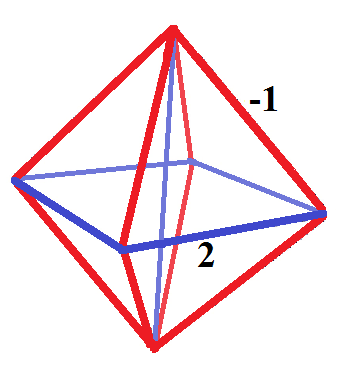
\includegraphics[width=70mm,scale=0.5]{newoctahedron.png}
\hspace{1.5cm}
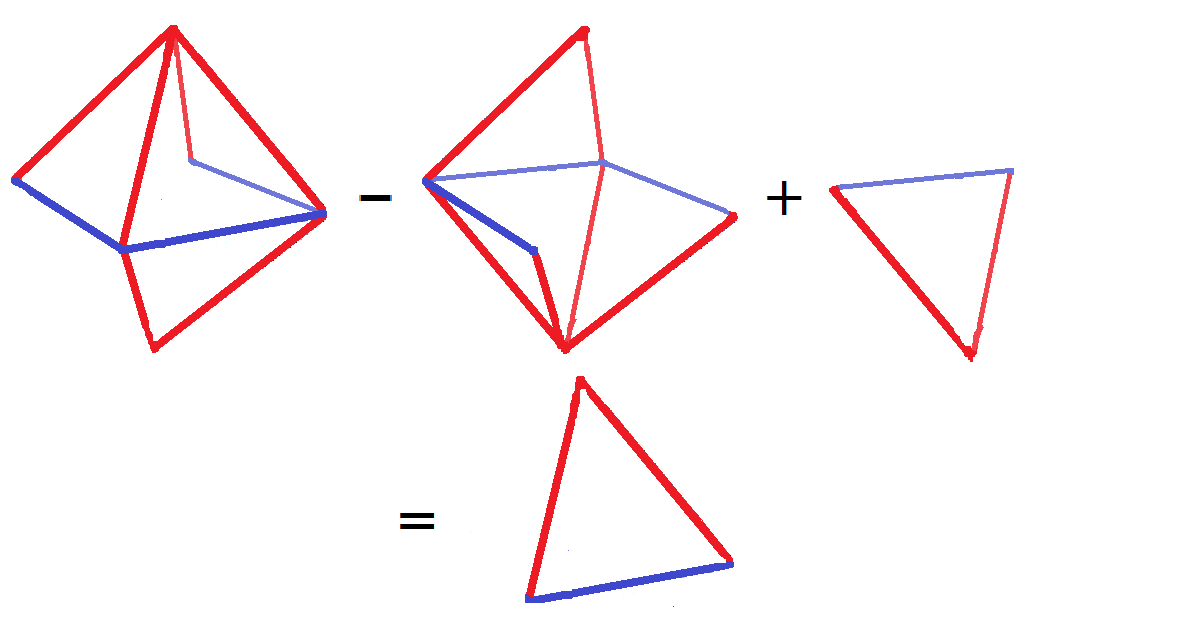
\includegraphics[width=150mm,scale=0.5]{newsumoctahedron.png}
\vspace{-20mm}
\caption{Octahedron(left) and resulting sum(right)}
\end{figure}

}
\end{textblock}  

\begin{textblock}{4.2}(22.3,8.8)
\large{This octohedron give us the sum also depicted in figure 6 where we can construct one triangle from the other triangles in the octohedron. This gives that, upon incramention of $a_1$ in the facet (as in case 1), we don't lose more then $1$ dimension implying a trivial adjacency. \hfill $\square$
}
\end{textblock}

\begin{textblock}{5.5}(16.8,11.1)
\large{Not restricting to these two cases, what happens in an arbitrary graph that has every edge in at least two vanishing triangle is still an open question. It seems from the data that most facets fall into these two cases. However, figure 7 gives examples of facet normals that don't. The cases at least give a characterization of adjacency structure. Future research should 
look both at the further simplification of the cone via adjacencies and at the application of the cone to the Nash-Williams conjecture. 
}
\end{textblock} 

\begin{textblock}{3}(23,11.2)
\begin{figure}
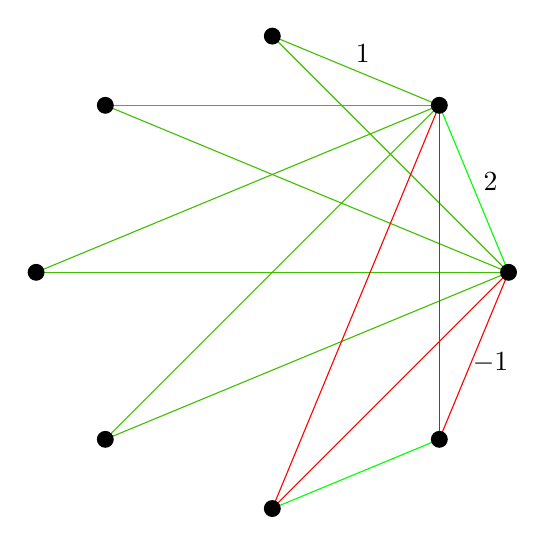
\begin{tikzpicture}
\node at ( 2.772 , 1.148 ){$ 2 $};
\draw[green! 100.0 !red] ( 3.0 , 0.0 )--( 2.121 , 2.121 );
\draw[green! 75.0 !red] ( 3.0 , 0.0 )--( 0.0 , 3.0 );
\node at ( 1.148 , 2.772 ){$ 1 $};
\draw[green! 75.0 !red] ( 2.121 , 2.121 )--( 0.0 , 3.0 );
\draw[green! 75.0 !red] ( 3.0 , 0.0 )--( -2.121 , 2.121 );
\draw[green! 75.0 !red] ( 2.121 , 2.121 )--( -2.121 , 2.121 );
\draw[green! 75.0 !red] ( 3.0 , 0.0 )--( -3.0 , 0.0 );
\draw[green! 75.0 !red] ( 2.121 , 2.121 )--( -3.0 , 0.0 );
\draw[green! 75.0 !red] ( 3.0 , 0.0 )--( -2.121 , -2.121 );
\draw[green! 75.0 !red] ( 2.121 , 2.121 )--( -2.121 , -2.121 );
\draw[red! 100.0 !green] ( 3.0 , 0.0 )--( 0.0 , -3.0 );
\draw[red! 100.0 !green] ( 2.121 , 2.121 )--( 0.0 , -3.0 );
\node at ( 2.772 , -1.148 ){$ -1 $};
\draw[red! 100.0 !green] ( 3.0 , 0.0 )--( 2.121 , -2.121 );
\draw[red! 100.0 !green] ( 2.121 , 2.121 )--( 2.121 , -2.121 );
\draw[green! 100.0 !red] ( 0.0 , -3.0 )--( 2.121 , -2.121 );
\filldraw ( 3.0 , 0.0 ) circle [radius=.1];
\filldraw ( 2.121 , 2.121 ) circle [radius=.1];
\filldraw ( 0.0 , 3.0 ) circle [radius=.1];
\filldraw ( -2.121 , 2.121 ) circle [radius=.1];
\filldraw ( -3.0 , 0.0 ) circle [radius=.1];
\filldraw ( -2.121 , -2.121 ) circle [radius=.1];
\filldraw ( 0.0 , -3.0 ) circle [radius=.1];
\filldraw ( 2.121 , -2.121 ) circle [radius=.1];
\end{tikzpicture}
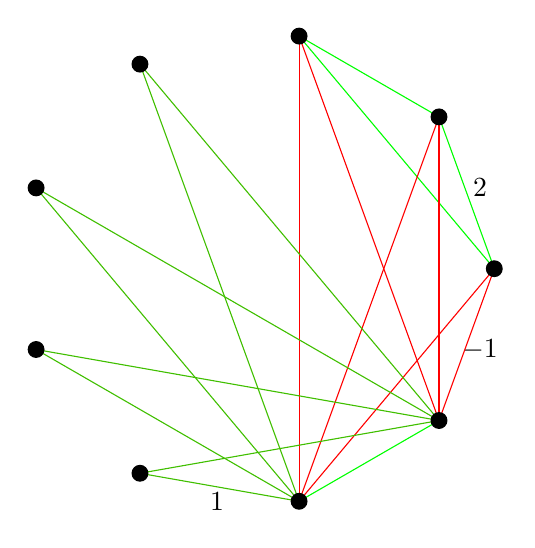
\begin{tikzpicture}
\node at ( 2.819 , 1.026 ){$ 2 $};
\draw[green! 100.0 !red] ( 3.0 , 0.0 )--( 2.298 , 1.928 );
\draw[green! 100.0 !red] ( 3.0 , 0.0 )--( 0.521 , 2.954 );
\draw[green! 100.0 !red] ( 2.298 , 1.928 )--( 0.521 , 2.954 );
\draw[red! 100.0 !green] ( 3.0 , 0.0 )--( 0.521 , -2.954 );
\draw[red! 100.0 !green] ( 2.298 , 1.928 )--( 0.521 , -2.954 );
\draw[red! 100.0 !green] ( 0.521 , 2.954 )--( 0.521 , -2.954 );
\draw[green! 75.0 !red] ( -1.5 , 2.598 )--( 0.521 , -2.954 );
\draw[green! 75.0 !red] ( -2.819 , 1.026 )--( 0.521 , -2.954 );
\draw[green! 75.0 !red] ( -2.819 , -1.026 )--( 0.521 , -2.954 );
\node at ( -0.521 , -2.954 ){$ 1 $};
\draw[green! 75.0 !red] ( -1.5 , -2.598 )--( 0.521 , -2.954 );
\node at ( 2.819 , -1.026 ){$ -1 $};
\draw[red! 100.0 !green] ( 3.0 , 0.0 )--( 2.298 , -1.928 );
\draw[red! 100.0 !green] ( 2.298 , 1.928 )--( 2.298 , -1.928 );
\draw[red! 100.0 !green] ( 0.521 , 2.954 )--( 2.298 , -1.928 );
\draw[green! 75.0 !red] ( -1.5 , 2.598 )--( 2.298 , -1.928 );
\draw[green! 75.0 !red] ( -2.819 , 1.026 )--( 2.298 , -1.928 );
\draw[green! 75.0 !red] ( -2.819 , -1.026 )--( 2.298 , -1.928 );
\draw[green! 75.0 !red] ( -1.5 , -2.598 )--( 2.298 , -1.928 );
\draw[green! 100.0 !red] ( 0.521 , -2.954 )--( 2.298 , -1.928 );
\filldraw ( 3.0 , 0.0 ) circle [radius=.1];
\filldraw ( 2.298 , 1.928 ) circle [radius=.1];
\filldraw ( 0.521 , 2.954 ) circle [radius=.1];
\filldraw ( -1.5 , 2.598 ) circle [radius=.1];
\filldraw ( -2.819 , 1.026 ) circle [radius=.1];
\filldraw ( -2.819 , -1.026 ) circle [radius=.1];
\filldraw ( -1.5 , -2.598 ) circle [radius=.1];
\filldraw ( 0.521 , -2.954 ) circle [radius=.1];
\filldraw ( 2.298 , -1.928 ) circle [radius=.1];
\end{tikzpicture}
\caption{Outlier facet normals}
\end{figure}
\end{textblock}


\begin{textblock}{9.7}(16.8,13.5)
\LARGEhead{References}
\vspace*{-4cm}
\begin{thebibliography}{99}
\bibitem{Nash-Will} C.S.J. Nash-Williams. An unsolved problem concerning decomposition of graphs into triangles. \textit{Combinatorial Theory and its Applications III}, pages 1179-1183, 1970.

\bibitem{Dross} F. Dross, Fractional triangle decompositions in graphs with
large minimum degree, 2015, v3, arXiv:1503.08191.
\end{thebibliography}

\bibliographystyle{unsrt}
\bibliography{facetposter}

\vspace{-5mm}

%%%%% END OF CONTENT %%%%%%%
\LARGEhead{Supervisor}
\Large{: Dr. Peter Dukes}
\end{textblock}

\end{document}
